\section{Inverse Scattering Time Analysis}

We hace derived the inverse scattering time matrix element from previous section as follows
\begin{equation} \label{5.1}
  \begin{aligned}
    \qty(\frac{1}{\tau(\varepsilon,k_x)})^{ll'}_{N} =
    \frac { N_{imp}^2 A^2 \hbar V_{imp}}{16\pi^4 \qty(eB)^2}
    \delta(\varepsilon - \varepsilon_{N})
    \int_{-\infty}^{\infty} d {k'}_x
    &
    J_l\qty(\frac{g\hbar}{eB}[{k}_x - {k'}_x])
    J_{l'}\qty(\frac{g\hbar}{eB}[{k}_x - {k'}_x]) \\
    & \times
    \qty|
    \int_{-\infty}^{\infty} d\bar{k} \;
    {\chi}_{N}\qty(\frac{\hbar}{eB}\bar{k})
    {\chi}_{N}\qty(\frac{\hbar}{eB} \qty[{k'}_x - {k}_x - \bar{k}])|^2.
  \end{aligned}
\end{equation}

\noindent
The disorder in the system is not supposed to change the eigenenergies of the bare system, hence all off-diogonal elements of the self-energy were neglected. Thesefore we can consider only the central diagonal element (${l=l'=0}$) of the inverse scattering time matrix which has the largest contribution
\begin{equation} \label{5.2}
  \begin{aligned}
    \qty(\frac{1}{\tau(\varepsilon,k_x)})^{00}_{N} =
    \frac { N_{imp}^2 A^2 \hbar V_{imp}}{16\pi^4 \qty(eB)^2}
    \delta(\varepsilon - \varepsilon_{N}) &
    \int_{-\infty}^{\infty} d {k'}_x \;
    J_l^2\qty(\frac{g\hbar}{eB}[{k}_x - {k'}_x])
    \\
    & \times
    \qty|
    \int_{-\infty}^{\infty} d\bar{k} \;
    {\chi}_{N}\qty(\frac{\hbar}{eB}\bar{k})
    {\chi}_{N}\qty(\frac{\hbar}{eB} \qty[{k'}_x - {k}_x - \bar{k}])|^2.
  \end{aligned}
\end{equation}

% and introduce new variable as follows
% \begin{equation} \label{5.3}
%     y_1 = \frac{\hbar}{eB}[{k'}_x - k_x] \longrightarrow
%     d{k'}_x = \frac{eB}{\hbar}dy_1
% \end{equation}
% and
% \begin{equation} \label{5.4}
%     y_2 = \frac{\hbar}{eB}\bar{k} \longrightarrow
%     d\bar{k} = \frac{eB}{\hbar}dy_2
% \end{equation}
% then above equation modified to
% \begin{equation} \label{5.5}
%   \begin{aligned}
%     \qty(\frac{1}{\tau(\varepsilon,k_x)})^{ll}_{N} =
%     \frac { N_{imp}^2 A^2 \hbar V_{imp}}{16\pi^4 \qty(eB)^2}
%     \qty(\frac{eB}{\hbar})^3
%     \delta(\varepsilon - \varepsilon_{N}) &
%     \int_{-\infty}^{\infty} dy_1\;
%     J_l^2\qty(\frac{g\hbar}{eB}[{k}_x - {k'}_x])
%     \\
%     & \times
%     \qty|
%     \int_{-\infty}^{\infty} d\bar{k} \;
%     {\chi}_{n_{\beta}}\qty(\frac{\hbar}{eB}\bar{k})
%   \end{aligned}
% \end{equation}

% \noindent
% Lets consider how this expression change when we have turn off the dressing field ($E = 0$). Thesefore the inverse scattering time becomes valid for only $l=0$
% \begin{equation} \label{5.3}
%   \begin{aligned}
%     \qty(\frac{1}{\tau(\varepsilon,k_x)})^{00}_{N}\Bigg|_{E=0}  =
%     \frac { N_{imp}^2 A^2 \hbar V_{imp}}{16\pi^4 \qty(eB)^2}
%     \delta(\varepsilon - \varepsilon_{N})
%     \int_{-\infty}^{\infty} d {k'}_x \;
%     \qty|
%     \int_{-\infty}^{\infty} d\bar{k} \;
%     {\chi}_{N}\qty(\frac{\hbar}{eB}\bar{k})
%     {\chi}_{N}\qty(\frac{\hbar}{eB} \qty[{k'}_x - {k}_x - \bar{k}])|^2.
%   \end{aligned}
% \end{equation}

\noindent
Now we can introduce a new parameter with physical meaning of scatterin-induced broadening of the Landau level as follows
\begin{equation} \label{5.3}
  \Gamma^{00}_{N}(\varepsilon,k_x) \equiv \hbar \qty(\frac{1}{\tau(\varepsilon,k_x)})^{00}_{N}
\end{equation}
and this modify our previous expressing as
\begin{equation} \label{5.4}
  \begin{aligned}
    \Gamma^{00}_{N}(\varepsilon,k_x)  =
    \frac { N_{imp}^2 A^2 \hbar^2 V_{imp}}{16\pi^4 \qty(eB)^2}
    \delta(\varepsilon - \varepsilon_{N}) &
    \int_{-\infty}^{\infty} d {k'}_x \;
    J_0^2\qty(\frac{g\hbar}{eB}[{k}_x - {k'}_x])
    \\
    & \times
    \qty|
    \int_{-\infty}^{\infty} d\bar{k} \;
    {\chi}_{N}\qty(\frac{\hbar}{eB}\bar{k})
    {\chi}_{N}\qty(\frac{\hbar}{eB} \qty[{k'}_x - {k}_x - \bar{k}])|^2.
  \end{aligned}
\end{equation}
In addition, for the case of elastic scattering within the same Landau level, one can present the delta distribution of the energy using the same physical interpretation as follows
\begin{equation} \label{5.5}
  \delta(\varepsilon - \varepsilon_{N}) \approx
  \frac{1}{\pi \Gamma^{00}_{N}(\varepsilon,k_x)}
\end{equation}
and this leads to
\begin{equation} \label{5.6}
  \begin{aligned}
    \qty[\Gamma^{00}_{N}(\varepsilon,k_x)]^2  =
    \frac { N_{imp}^2 A^2 \hbar^2 V_{imp}}{16\pi^5 \qty(eB)^2}
    \int_{-\infty}^{\infty} d {k'}_x \;
    J_0^2\qty(\frac{g\hbar}{eB}[{k}_x - {k'}_x])
    \qty|
    \int_{-\infty}^{\infty} d\bar{k} \;
    {\chi}_{N}\qty(\frac{\hbar}{eB}\bar{k})
    {\chi}_{N}\qty(\frac{\hbar}{eB} \qty[{k'}_x - {k}_x - \bar{k}])|^2.
  \end{aligned}
\end{equation}
and
\begin{equation} \label{5.7}
  \begin{aligned}
    \Gamma^{00}_{N}(\varepsilon,k_x)  =
    \qty[
    \frac { N_{imp}^2 A^2 \hbar^2 V_{imp}}{16\pi^5 \qty(eB)^2}
    \int_{-\infty}^{\infty} d {k'}_x \;
    J_0^2\qty(\frac{g\hbar}{eB}[{k}_x - {k'}_x])
    \qty|
    \int_{-\infty}^{\infty} d\bar{k} \;
    {\chi}_{N}\qty(\frac{\hbar}{eB}\bar{k})
    {\chi}_{N}\qty(\frac{\hbar}{eB} \qty[{k'}_x - {k}_x - \bar{k}])|^2
    ]^{-1/2}.
  \end{aligned}
\end{equation}

\noindent
This can be write in more compact form as follows
\begin{equation} \label{5.8}
  \begin{aligned}
    \Gamma^{00}_{N}(\varepsilon,k_x)  =
    \qty[
    \frac { N_{imp}^2 A^2 \hbar^2 V_{imp}}{16\pi^5 \qty(eB)^2}
    \int_{-\infty}^{\infty} d {k'}_x \;
    J_0^2\qty(g\sigma[{k}_x - {k'}_x])
    \qty|
    \int_{-\infty}^{\infty} d\bar{k} \;
    {\chi}_{N}\qty(\sigma\bar{k})
    {\chi}_{N}\qty(\sigma\qty[{k'}_x - {k}_x - \bar{k}])|^2
    ]^{-1/2}
  \end{aligned}
\end{equation}
where
\begin{equation} \label{5.9}
    g = \frac{eE\omega_0^2}{\hbar\omega(\omega_0^2 - \omega^2)} \quad\quad
    \sigma = \frac{\hbar}{eB}
\end{equation}
and
\begin{equation} \label{5.10}
  \chi_N(x) = \frac{\sqrt{\kappa}}{\sqrt{2^{N}N!\sqrt{\pi}}}
  \exp(-\frac{\kappa^2 x^2}{2})
  \mathcal{H}_N\qty(\kappa x) \quad \text{with} \quad
  \kappa \equiv \sqrt{\frac{m_e \omega_0}{\hbar}}.
\end{equation}

\noindent
Using above definition we can identify Gauss-Hermite functions ($\tilde{\chi}_N$) and this can re-write as
\begin{equation} \label{5.11}
  \begin{aligned}
    \Gamma^{00}_{N}(\varepsilon,k_x)  =
    \qty[
    \frac { N_{imp}^2 A^2 \hbar^2 V_{imp} \kappa^4}{16\pi^5 \qty(eB)^2}
    \int_{-\infty}^{\infty} d {k'}_x \;
    J_0^2\qty(g\sigma[{k}_x - {k'}_x])
    \qty|
    \int_{-\infty}^{\infty} d\bar{k} \;
    \tilde{\chi}_{N}\qty(\sigma\kappa\bar{k})
    \tilde{\chi}_{N}\qty(\sigma\kappa\qty[{k'}_x - {k}_x - \bar{k}])|^2
    ]^{-1/2}
  \end{aligned}
\end{equation}
where
\begin{equation} \label{5.12}
  \tilde{\chi}_N(x) = \frac{1}{\sqrt{2^{N}N!\sqrt{\pi}}}
  \exp(-\frac{x^2}{2})
  \mathcal{H}_N\qty(x)
\end{equation}
and this will be simplified to
\begin{equation} \label{5.13}
  \begin{aligned}
    \Gamma^{00}_{N}(\varepsilon,k_x)  =
    \eta
    \qty[
    \int_{-\infty}^{\infty} d {k}_1 \;
    J_0^2\qty(\lambda_1[{k}_x - {k}_1])
    \qty|
    \int_{-\infty}^{\infty} d{k}_2 \;
    \tilde{\chi}_{N}\qty(\lambda_2 k_2)
    \tilde{\chi}_{N}\qty(\lambda_2 \qty[{k}_1 - {k}_2 - {k}_x])|^2
    ]^{-1/2}
  \end{aligned}
\end{equation}
where
\begin{equation} \label{5.14}
    \eta = \qty[\frac { N_{imp}^2 A^2 V_{imp}}{16\pi^5}]^{1/2} \quad,\quad
    \lambda_1 = g\sigma \quad,\quad
    \lambda_2 = \sigma \kappa.
\end{equation}
\noindent
Now we can analyze the behaviour of the normalized $N$-th Landau level for broadening as follows
\begin{equation} \label{5.15}
    \Lambda_N(k_x) \equiv
    \frac{\qty(1/\tau)^{00}_{N}}{\qty(1/\tau)^{00}_{0}\big|_{E=0}} =
    \frac{\Gamma^{00}_{N}(\varepsilon,k_x)}{\Gamma^{00}_{0}(\varepsilon,k_x)\big|_{E=0}}
\end{equation}
and this will be
\begin{equation} \label{5.16}
    \Lambda_N (k_x) =
    \qty[
    \frac
    {\int_{-\infty}^{\infty} d {k}_1 \;
    J_0^2\qty(\lambda_1[{k}_x - {k}_1])
    \qty|
    \int_{-\infty}^{\infty} d{k}_2 \;
    \tilde{\chi}_{N}\qty(\lambda_2 k_2)
    \tilde{\chi}_{N}\qty(\lambda_2 \qty[{k}_1 - {k}_2 - {k}_x])|^2}
    {\int_{-\infty}^{\infty} d {k}_1 \;
    \qty|
    \int_{-\infty}^{\infty} d{k}_2 \;
    \tilde{\chi}_{0}\qty(\lambda_2 k_2)
    \tilde{\chi}_{0}\qty(\lambda_2 \qty[{k}_1 - {k}_2 - {k}_x])|^2}
    ]^{1/2}.
\end{equation}

\noindent
Lets calculate these constants for GaAs-based quantum well with following given physical constants and system external paramters.

\begin{table}[ht!]
\begin{center}
\begin{tabular}{ |l|c|l| }
 \hline
 \textbf{Physical constant name} & \textbf{Symbol} & \textbf{Value in SI-units} \\ [0.5ex] \hline\hline
 Electron charge  & e & $1.602\times10^{-19} \;\text{C}$ \\ \hline
 Electron mass & $m$ & $9.109\times10^{-31}\; \text{kg}$ \\ \hline
 Reduced Planck's constant &  $\hbar$ & $1.054\times10^{-34} \;\text{kg}\text{m}^2\text{s}^{-1}$ \\ \hline
 Speed of light & $c$ & $2.998\times10^8\; \text{ms}^{-1}$ \\ \hline
 Vacuum permittivity & $\varepsilon_0$ & $8.854\times10^{-12}\; \text{C}^{2}\text{s}^2\text{kg}^{-1}\text{m}^{-3}$ \\ \hline
\end{tabular}
\caption {\label{tab:5.1}Physical constant values in SI-units}
\end{center}
\end{table}

\begin{table}[ht!]
\begin{center}
\begin{tabular}{ |l|c|l| }
 \hline
 \textbf{External paramter name} & \textbf{Symbol} & \textbf{Value in SI-units} \\ [0.5ex] \hline\hline
 Average intensity  & $I$ & $\tilde{I} \times 100\;\text{W}/\text{cm}^{2} = \tilde{I}\times10^6\;\text{W}/\text{m}^{2}$ \\ \hline
 Magnetic field & $B$ & $1.2\;\text{T}$ \\ \hline
 Driving frequency & $\omega$ & $2\times10^{12} \;\text{rad}\text{s}^{-1}$ \\ \hline
 Effective mass &  $m_e$ & $0.071\times m = 6.467 \times10^{-32} \; \text{kg}$ \\ \hline
\end{tabular}
\caption {\label{tab:5.2}System external paramter values. (${\tilde{I}}$ is a dimentionless value.)}
\end{center}
\end{table}

\noindent
Therfore we can calculate following values
\begin{equation} \label{5.17}
  \omega_0 = \frac{eB}{m_e} = 2.97265 \times 10^{12}\; \text{s}^{-1}
\end{equation}
\begin{equation} \label{5.18}
  \sigma = \frac{\hbar}{eB} = 5.4851 \times 10^{-16}\; \text{m}^{2}
\end{equation}
\begin{equation} \label{5.19}
  E = \sqrt{\frac{2I}{c\varepsilon_0}}
\end{equation}
\begin{equation} \label{5.20}
  g = \frac{eE\omega_0^2}{\hbar\omega(\omega_0^2 - \omega^2)}
  = \frac{e\omega_0^2}{\hbar\omega(\omega_0^2 - \omega^2)}  \sqrt{\frac{2I}{c\varepsilon_0}}
  = 3.80958 \times 10^{7}\times \sqrt{\tilde{I}}\; \text{m}^{-1}
\end{equation}
\begin{equation} \label{5.21}
  \kappa = \sqrt{\frac{m_e \omega_0}{\hbar}}
  = 4.2698 \times 10^{7}\; \text{m}^{-1}
\end{equation}
Since
\begin{equation} \label{5.22}
  \lambda_1 = g\sigma
  = 2.08959 \times 10^{-8} \times \sqrt{\tilde{I}}\; \text{m} \quad \text{and} \quad
  \lambda_2 = \kappa\sigma = 2.34203 \times 10^{-8}\; \text{m}
\end{equation}
we can choose our integral dummy variables $k_1$, $k_2$ and momentum variable $k_x$ are in one range as follows
\begin{equation} \label{5.23}
  k_x,k_1,k_2 \approx 10^{8}\; \text{m}^{-1}
\end{equation}

\noindent
Using above values we can re-write the normalized energy broadening of the $N$-th Landau level as
\begin{equation} \label{5.24}
    \Lambda_N (k_x) =
    \qty[
    \frac
    {\int_{-\infty}^{\infty} d {k}_1 \;
    J_0^2\qty(2.090\sqrt{\tilde{I}}\times[{k}_x - {k}_1])
    \qty|
    \int_{-\infty}^{\infty} d{k}_2 \;
    \tilde{\chi}_{N}\qty(2.342 \times k_2)
    \tilde{\chi}_{N}\qty(2.342 \times \qty[{k}_1 - {k}_2 - {k}_x])|^2}
    {\int_{-\infty}^{\infty} d {k}_1 \;
    \qty|
    \int_{-\infty}^{\infty} d{k}_2 \;
    \tilde{\chi}_{0}\qty(2.342 \times k_2)
    \tilde{\chi}_{0}\qty(2.342 \times \qty[{k}_1 - {k}_2 - {k}_x])|^2}
    ]^{1/2}.
\end{equation}
\begin{figure}[ht!]
  \centering
  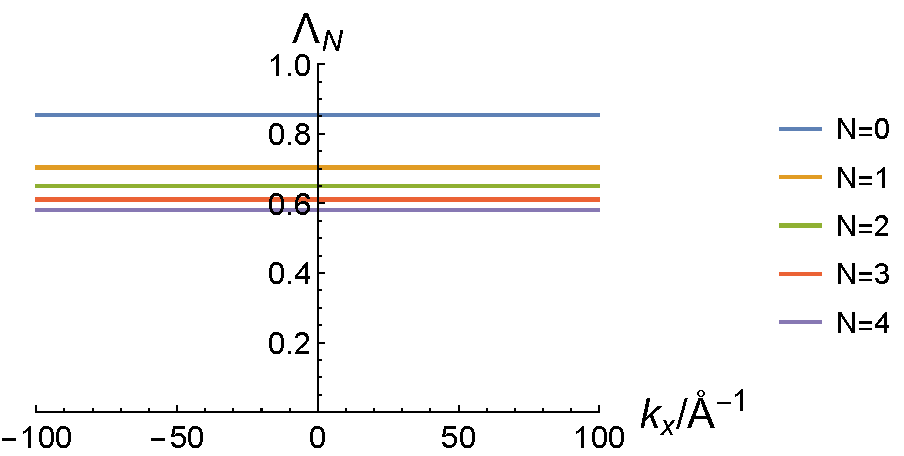
\includegraphics[scale=0.7]{figures/fig51.pdf}
  \caption{Normalized energy band broadening with $k_x$ for different Landau levels ($N=0,1,2,3,4$) for $\tilde{I}=1$.}
  \label{fig:5.1}
\end{figure}

\noindent
To check the variability of this expression with $k_x$ value we check it with a constant intensity. Therefore let $\tilde{I}=1$ and we can re-write above as
\begin{equation} \label{5.25}
    \Lambda_N (k_x) =
    \qty[
    \frac
    {\int_{-\infty}^{\infty} d {k}_1 \;
    J_0^2\qty(2.090\times[{k}_x - {k}_1])
    \qty|
    \int_{-\infty}^{\infty} d{k}_2 \;
    \tilde{\chi}_{N}\qty(2.342 \times k_2)
    \tilde{\chi}_{N}\qty(2.342 \times \qty[{k}_1 - {k}_2 - {k}_x])|^2}
    {\int_{-\infty}^{\infty} d {k}_1 \;
    \qty|
    \int_{-\infty}^{\infty} d{k}_2 \;
    \tilde{\chi}_{0}\qty(2.342 \times k_2)
    \tilde{\chi}_{0}\qty(2.342 \times \qty[{k}_1 - {k}_2 - {k}_x])|^2}
    ]^{1/2}.
\end{equation}
then introduce new variable
\begin{equation} \label{5.26}
  k_1 - k_x = \tilde{k} \quad \longrightarrow \quad dk_1 = d\tilde{k}
\end{equation}
and since $k_1$ can vary between all the range we can modify our Eq. \eqref{5.25} as follows
\begin{equation} \label{5.27}
    \Lambda_N (k_x) =
    \qty[
    \frac
    {\int_{-\infty}^{\infty} d \tilde{k} \;
    J_0^2\qty(2.090\times \tilde{k})
    \qty|
    \int_{-\infty}^{\infty} d{k}_2 \;
    \tilde{\chi}_{N}\qty(2.342 \times k_2)
    \tilde{\chi}_{N}\qty(2.342 \times \qty[\tilde{k}- {k}_2])|^2}
    {\int_{-\infty}^{\infty} d \tilde{k} \;
    \qty|
    \int_{-\infty}^{\infty} d{k}_2 \;
    \tilde{\chi}_{0}\qty(2.342 \times k_2)
    \tilde{\chi}_{0}\qty(2.342 \times \qty[\tilde{k} - {k}_2])|^2}
    ]^{1/2}
\end{equation}
and letting $\tilde{k} = k_1$ we can find that this is do not depend on the value of $k_x$. Therefore
\begin{equation} \label{5.28}
    \Lambda_N =
    \qty[
    \frac
    {\int_{-\infty}^{\infty} d k_1 \;
    J_0^2\qty(2.090\times k_1)
    \qty|
    \int_{-\infty}^{\infty} d{k}_2 \;
    \tilde{\chi}_{N}\qty(2.342 \times k_2)
    \tilde{\chi}_{N}\qty(2.342 \times \qty[k_1 - {k}_2])|^2}
    {\int_{-\infty}^{\infty} d k_1\;
    \qty|
    \int_{-\infty}^{\infty} d{k}_2 \;
    \tilde{\chi}_{0}\qty(2.342 \times k_2)
    \tilde{\chi}_{0}\qty(2.342 \times \qty[k_1 - {k}_2])|^2}
    ]^{1/2}
\end{equation}

\noindent
Now we can draw the values of $\Lambda_N$ agaist $k_x$ to compare the differese of each Landau level's normalized energy band broadening as given in Figure \ref{fig:5.1}.

\noindent
Now let's check how the $\Lambda_N$ value change with the applied dressing field's intensity. Using following equation we can identify $\Lambda_N$ dependency on dressing field's intensity as given in Figure \ref{fig:5.2}.
\begin{equation} \label{5.29}
    \Lambda_N  =
    \qty[
    \frac
    {\int_{-\infty}^{\infty} d {k}_1 \;
    J_0^2\qty(2.090\sqrt{\tilde{I}}\times{k}_1)
    \qty|
    \int_{-\infty}^{\infty} d{k}_2 \;
    \tilde{\chi}_{N}\qty(2.342 \times k_2)
    \tilde{\chi}_{N}\qty(2.342 \times \qty[{k}_1 - {k}_2])|^2}
    {\int_{-\infty}^{\infty} d {k}_1 \;
    \qty|
    \int_{-\infty}^{\infty} d{k}_2 \;
    \tilde{\chi}_{0}\qty(2.342 \times k_2)
    \tilde{\chi}_{0}\qty(2.342 \times \qty[{k}_1 - {k}_2])|^2}
    ]^{1/2}.
\end{equation}

\begin{figure}[ht!]
  \centering
  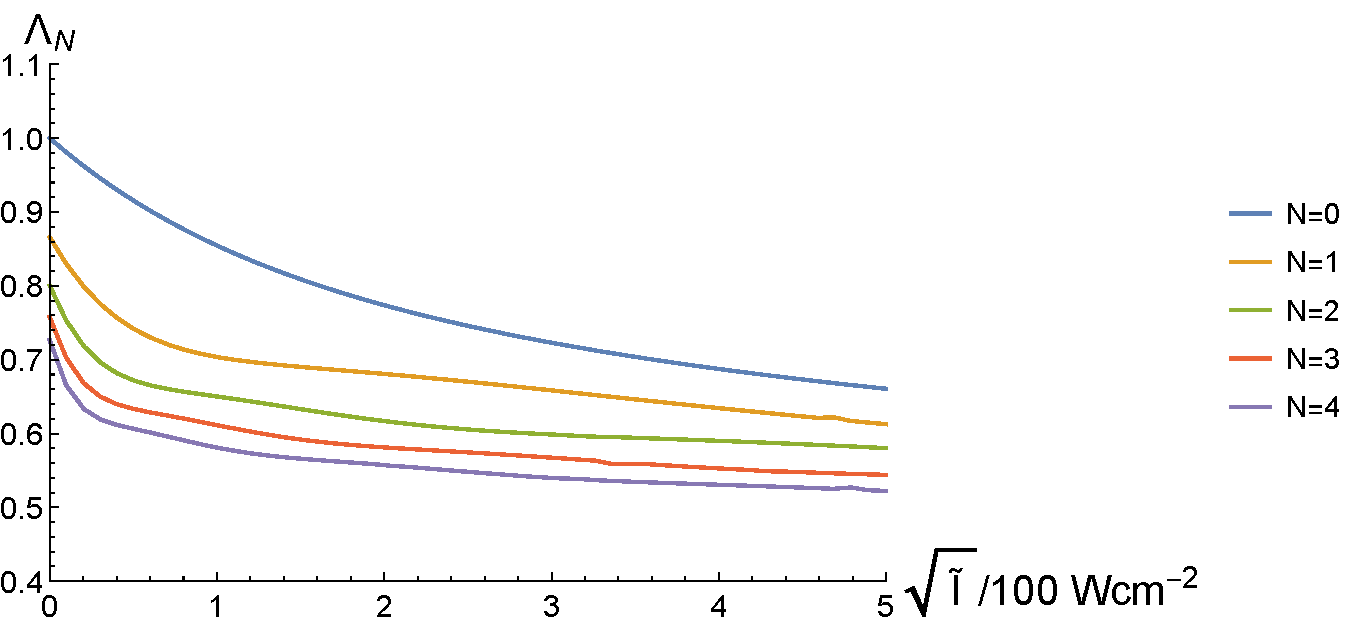
\includegraphics[scale=0.6]{figures/fig52.pdf}
  \caption{Normalized energy band broadening with $k_x$ for different Landau levels ($N=0,1,2,3,4$) for $\tilde{I}=1$.}
  \label{fig:5.2}
\end{figure}

\noindent
Here we can identify that we can change the each Landau level normalized energy broadening value using apllied electromagnetic field. When the applied field's intensity increase the energy broadening gets reduced which make changes in conductivity.

\noindent
To make comparison we can select the experiment parameters from previous analysis on transverse conductivity in [*Ref: Akira Endo and Naomichi Hantno]. In this study we have assumed that the broadening of Landau levels are same and the value for $\Gamma_N$ non-existing dressing field is $0.24\;\text{me}V$. Therefore in our study for the comparison we can assume that the least Landau level broadening has this value.
\begin{equation} \label{5.30}
  \Gamma^{00}_{N=0}\big|_{E=0} = 0.24 \;\text{meV}
\end{equation}

\noindent
Then using the calculated normalized broadening relations for each Landu levels, we can evaluate the energy band broadening values as follows
\begin{equation} \label{5.31}
  \Gamma^{00}_{N} = \Lambda_N \times \Gamma^{00}_{N=0}\big|_{E=0}.
\end{equation}
Therfore, the energy band broadening for Landau level with dressing field can be calculate as
\begin{equation} \label{5.32}
  \Gamma^{00}_{N} = \Lambda_N \times \Gamma^{00}_{N=0}\big|_{E=0}.
\end{equation}
and
\begin{equation} \label{5.33}
  \Gamma^{00}_{N} = 0.24 \times \Lambda_N  \;\text{meV}.
\end{equation}
\begin{equation} \label{5.34}
  \Gamma^{00}_{N}(\tilde{I}) = 0.24 \times
  \qty[
  \frac
  {\int_{-\infty}^{\infty} d {k}_1 \;
  J_0^2\qty(2.090\sqrt{\tilde{I}}\times{k}_1)
  \qty|
  \int_{-\infty}^{\infty} d{k}_2 \;
  \tilde{\chi}_{N}\qty(2.342 \times k_2)
  \tilde{\chi}_{N}\qty(2.342 \times \qty[{k}_1 - {k}_2])|^2}
  {\int_{-\infty}^{\infty} d {k}_1 \;
  \qty|
  \int_{-\infty}^{\infty} d{k}_2 \;
  \tilde{\chi}_{0}\qty(2.342 \times k_2)
  \tilde{\chi}_{0}\qty(2.342 \times \qty[{k}_1 - {k}_2])|^2}
  ]^{1/2} \text{meV}.
\end{equation}






























xx
